\chapter{系统需求分析}

\section{角色权限与权责划分}
在分析角色权限时，笔者主要还是从高校财务管理的实际业务出发。通过对 \texttt{SysUser\allowbreak Controller} 以及相关安全模块的梳理，系统将核心操作划分为科研人员与管理员两大类。这种划分配合 RBAC 模型的应用，能够在保证数据安全的前提下，让权责界限变得足够清晰，也为后续的流程管控提供了基础。

在具体分工上，科研人员主要负责项目层面的所有操作，包括申报信息、预算方案的编制，以及日常支出的报销申请。考虑到数据隐私，他们只能访问和修改自己负责的项目，并能通过风险中心接收系统推送的预警提醒。与此相对，管理员则拥有全局的数据视角，主要通过审核申报计划、报销单据来进行管理把控。为了提升决策效率，**我**专门为这类角色设计了全局看板，让他们能直观掌握所有项目的执行趋势，这比原本查表核对的方式效率要高得多。

\section{核心业务逻辑流程}
为了降低 \texttt{ResearchProject\allowbreak Service} 和 \texttt{FundExpenditure\allowbreak Service} 这些底层逻辑的耦合度，本研究将系统的核心业务梳理成了三条既相互关联、在流程上又保持独立的主线。

关于预算申报与核定，其核心任务是确保经费能精确拨付。系统通过状态机来驱动流程：科研人员录入的信息会先后经过“草稿”与“审核”状态，最终进入“待编制预算”这一关键节点。在此阶段，系统会执行强校验逻辑，各科目的预算总额必须与批复总额严格一致。如果金额对不上，流程就会被自动阻断，从而在源头上规避了账目错误的风险。

报销流程则是日常运作中最活跃的部分。每当有报销申请产生，系统都会去碰撞该科目目前的剩余额度，一旦发现超支就会立即进行拦截。报销单提交后会进入管理员的审核队列，管理员根据附件证据及其与预算的符合度给出最终结论。审核通过后，系统不仅会自动扣减余额，还会同步更新多维分析模型中的明细数据。

至于多维数据预警，它构成了系统辅助决策的闭环。系统后台通过定时任务与统计服务（\texttt{FundStatistics\allowbreak Service}）保持联动，实时扫描所有执行中的项目。分析的维度主要集中在时间进度、执行率以及结题期限等指标。如果系统捕捉到潜在风险，就会自动生成标识性的“智能风险标签”，通过这种自动监控代替人工盯防，极大地减轻了管理人员的压力\cite{Gaftandzhieva2023}。

\section{用例分析与交互建模}
在系统设计阶段，本课题利用 UML 用例图定义了功能的边界。虽然常规的用例分析往往侧重功能列举，但在设计过程中，笔者更关注业务交互的实质。

科研人员的交互主要集中在执行侧。从初始化申报到后续的报销和结题，每一个用例都在驱动系统状态的变更。为了保障数据的源头质量，**我**在这些输入环节增加了多层校验逻辑，防止一些明显的错误数据对后续的决策分析产生干扰。

管理员的用例则更倾向于宏观的管控。除了必要的审核功能，最核心的其实是“风险监控”与“决策查询”。管理员能够依据多维看板反馈的趋势，对异常项目进行快速介入。通过这种双向的交互逻辑，经费管理就不再是单向的数据填充，而是一个具备实时反馈能力的闭环体系。

\begin{figure}[htbp]
    \centering
    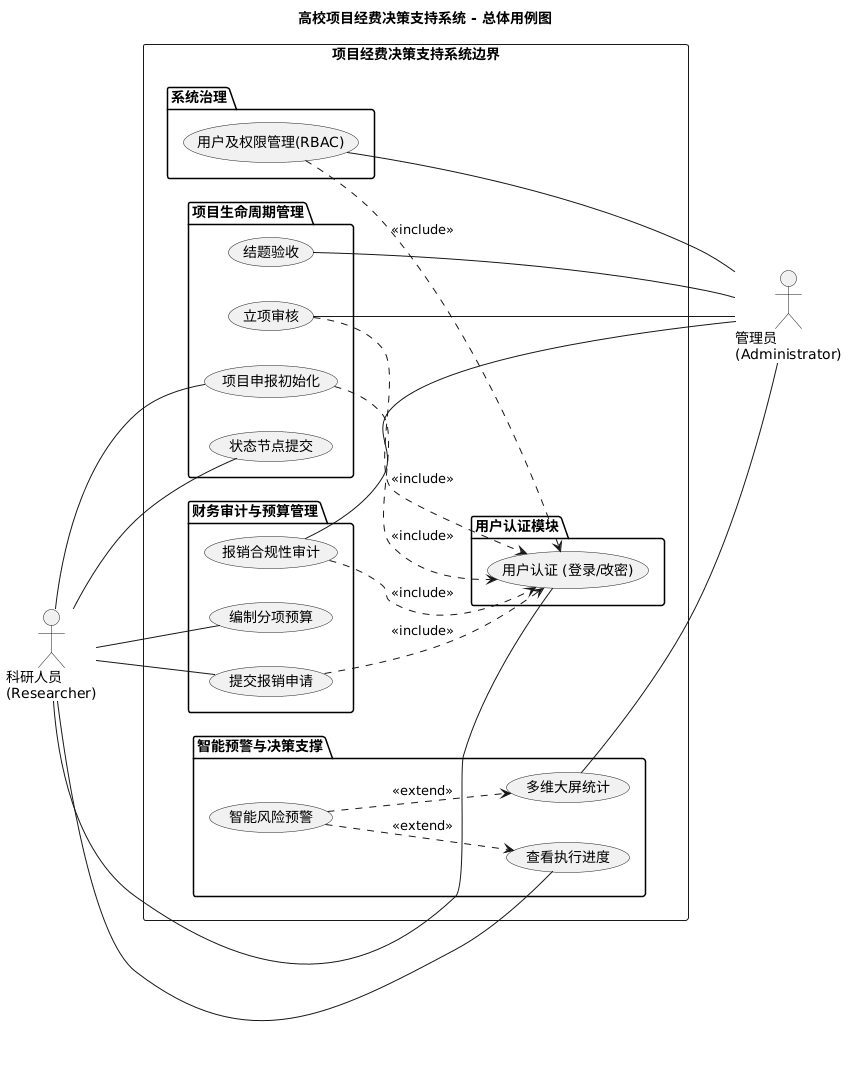
\includegraphics[width=0.8\textwidth]{figures/usecase.png}
    \caption{系统总体用例图}
    \label{fig:usecase}
\end{figure}

\section{系统功能与性能需求}
在明确系统需求时，本研究参考了戴建青等人的研究建议\cite{Dai2019}，并结合 \texttt{Controller} 层的业务场景，将系统的关键能力聚焦在了几个核心维度。

首先在业务管理层面，系统必须具备可靠的用户鉴权和全生命周期管理能力，确保从立项到结题的每一个状态位都能被准确维护。此外，精细化的科目配置也是必不可少的，系统应支持自定义科目并提供金额一致性的自动演算。而在数据分析层面，多维查询引擎和可视化看板则是系统的“灵魂”，它们负责将复杂的财务流水转化为直观的趋势图和风险汇总。

为了保证这些功能的稳健运行，本系统在安全、性能和可靠性方面也设定了相关标准。安全性方面，系统采用了基于 JWT 的认证与 BCrypt 的哈希加密，通过 Spring Security 建立了严密的权限防线。针对性能问题，考虑到多维分析的海量计算量，程序引入了数据快照（\texttt{FundStatistics\allowbreak Snapshot}）机制，将复杂的计算结果进行异步缓存。这种方式虽然会产生轻微的数据延迟，但极大地提升了查看看板时的流畅度。最后，在可靠性上，**我**利用声明式事务来保证财务操作的原子性，确保在任何意外情况下，账目都能实现准确的回滚。

\section{决策支持指标设计}
决策支持模块的“大脑”是基于时间与经费执行的交叉分析。这些指标的设计并没有追求过度复杂的数学建模，而是选择了最能反映问题的几个观测点。虽然阈值设定具有一定的经验性，但在实际演示中非常有效：

指标一：执行进度与时间进度的对冲分析。如果项目时间已经过半，但经费扣减比例仍远低于正常水平（差值超过 10\%），系统就会标记为“执行滞后”。这通常意味着项目任务可能遇到了瓶颈，或者报销流程出现了明显的积压。

指标二：单项预算的余额警戒。系统在每个科目上都设定了 90\% 的临界点。一旦某科目的开支接近这一比例，程序会立刻打上“告急”标签，提醒负责人提前规划预算调配。

指标三：结题倒计时的风险干预。系统会动态比对当前时间与预设的结题日，在最后的 20 天内，如果项目仍处于“执行中”状态，则会触发催促提醒，防止出现因延期导致的财务违规风险。
